\documentclass[12pt,a4paper]{article}

% Packages
\usepackage[utf8]{inputenc}
\usepackage[english]{babel}
\usepackage{amsmath,amssymb,amsthm}
\usepackage{graphicx}
\usepackage{geometry}
\usepackage{float}
\usepackage{caption}
\usepackage{subcaption}
\usepackage{hyperref}
\usepackage{siunitx}
\usepackage{booktabs}
\usepackage{bm}
\usepackage{tikz}
\usetikzlibrary{shapes.geometric, arrows.meta, positioning, fit, calc}
\usepackage{xcolor}

% Page geometry
\geometry{margin=2.5cm}

% Custom commands (same as main.tex)
\newcommand{\parder}[2]{\frac{\partial #1}{\partial #2}}
\newcommand{\pparder}[2]{\frac{\partial^2 #1}{\partial {#2}^2}}
\newcommand{\Rey}{\text{Re}}
\newcommand{\Pran}{\text{Pr}}

\begin{document}

% ============================================================================
% TITLE PAGE
% ============================================================================
\begin{titlepage}
    \centering
    \vspace*{2cm}

    {\Huge\bfseries Supplementary Derivations\par}

    \vspace{1cm}

    {\Large Cartesian and $(r,\phi)$ Cylindrical Coordinate Formulations\par}
    {\large --- Not Required by the Solved Assignment Problem ---\par}

    \vspace{1cm}

    {\large LV-Nr.: 321.053 EX\par}
    {\large Winter Semester 2025/26\par}

    \vfill

    {\Large
    Felix Scope\\
    \texttt{felix\_scope@yahoo.de}\\
    }

    \vfill

    {\large \today\par}
\end{titlepage}

\tableofcontents
\newpage

% ============================================================================
% PREFACE
% ============================================================================
\section*{Preface}
\addcontentsline{toc}{section}{Preface}

The graded assignment brief (\texttt{Assignment\_WS25.pdf}) asks, regarding
the theoretical derivation, only for the conservation equations of this 2D
flow problem to be formulated \emph{in cylindrical coordinates}
("\emph{Formulieren Sie die Erhaltungsgleichungen, welche dieses
zwei-dimensionale Str\"omungsproblem beschreiben, in Zylinderkoordinaten}").
The problem that was actually solved numerically -- entrance flow in a
cylindrical pipe -- is axisymmetric and uses the $(r,z)$ formulation with
velocities $(u,w)$. That derivation (governing equations, staggered-grid
layout, finite-volume discretisation, projection method, Poisson solver, and
ghost-cell boundary treatment), together with the MATLAB implementation and
results, is given in full in the main report (\texttt{main.pdf}, Appendix A).

The Cartesian $(x,y)$ and cylindrical $(r,\phi)$ derivations below go beyond
that brief. They follow a separate working note
(\texttt{Assignemnt/Derivations\_assignment}) that additionally called for
the same derivation method -- governing equations through ghost cells -- to
be carried out for 2D Cartesian $(x,y)$ and for 2D cylindrical $(r,\phi)$
with velocities $(u,v)$, alongside the $(r,z)$ case. Neither of these two
coordinate systems was ever solved numerically (no Cartesian domain and no
azimuthal/polar domain were part of the solver), so they are collected here,
separate from the main report, rather than in its appendix: the main
submission stays focused on the problem the graded brief actually asks for,
while this supplementary material remains available for reference.

\newpage

% ============================================================================
% APPENDIX-STYLE DERIVATIONS
% ============================================================================
% ============================================================
%  Derivation: 2D Cartesian Coordinates (x, y)
%  Velocities: u (x-direction), v (y-direction)
%  Integration element: dx dy
% ============================================================

\section{2D Incompressible Flow in Cartesian Coordinates $(x,y)$}
\label{sec:cartesian}

\subsection{Governing Equations (Strong Form)}

For a 2D incompressible Newtonian fluid with constant properties and no body forces:

\textbf{Continuity:}
\begin{equation}
    \frac{\partial u}{\partial x} + \frac{\partial v}{\partial y} = 0
    \label{eq:cart_cont}
\end{equation}

\textbf{$x$-momentum:}
\begin{equation}
    \frac{\partial u}{\partial t}
    + \frac{\partial(u^2)}{\partial x}
    + \frac{\partial(uv)}{\partial y}
    = -\frac{1}{\rho}\frac{\partial p}{\partial x}
    + \frac{1}{\rho}\frac{\partial\tau_{xx}}{\partial x}
    + \frac{1}{\rho}\frac{\partial\tau_{xy}}{\partial y}
    \label{eq:cart_momx}
\end{equation}

\textbf{$y$-momentum:}
\begin{equation}
    \frac{\partial v}{\partial t}
    + \frac{\partial(uv)}{\partial x}
    + \frac{\partial(v^2)}{\partial y}
    = -\frac{1}{\rho}\frac{\partial p}{\partial y}
    + \frac{1}{\rho}\frac{\partial\tau_{xy}}{\partial x}
    + \frac{1}{\rho}\frac{\partial\tau_{yy}}{\partial y}
    \label{eq:cart_momy}
\end{equation}

where for a Newtonian fluid with constant viscosity $\mu = \rho\nu$:
\begin{align}
    \tau_{xx} &= 2\mu\frac{\partial u}{\partial x}
    \\
    \tau_{yy} &= 2\mu\frac{\partial v}{\partial y}
    \\
    \tau_{xy} &= \mu\!\left(\frac{\partial u}{\partial y}+\frac{\partial v}{\partial x}\right)
\end{align}

\textbf{Conservation vs.\ Convective Form:}
The equations above are written in \emph{conservation form}, where momentum fluxes appear explicitly as divergences (e.g.\ $\frac{\partial(u^2)}{\partial x}$ and $\frac{\partial(uv)}{\partial y}$). This differs from the \emph{convective form}, which expands the nonlinear terms using the product rule. To derive the convective form, expand the momentum flux divergences:
\begin{equation}
    \frac{\partial(u^2)}{\partial x} + \frac{\partial(uv)}{\partial y}
    = u\frac{\partial u}{\partial x} + u\frac{\partial u}{\partial x} + v\frac{\partial u}{\partial y} + u\frac{\partial v}{\partial y}
    = u\left(\frac{\partial u}{\partial x} + \frac{\partial v}{\partial y}\right) + u\frac{\partial u}{\partial x} + v\frac{\partial u}{\partial y}
\end{equation}
By the continuity equation $\frac{\partial u}{\partial x} + \frac{\partial v}{\partial y} = 0$, the first grouped term vanishes, leaving:
\begin{equation}
    \frac{\partial(u^2)}{\partial x} + \frac{\partial(uv)}{\partial y} = u\frac{\partial u}{\partial x} + v\frac{\partial u}{\partial y}
\end{equation}
This is the **convective form**. The conservation form is preferable for numerical schemes because it naturally encodes momentum balance at each cell: the divergence operators directly represent net flux in and out of the control volume, which the finite volume method integrates over CV boundaries. The convective form, while mathematically equivalent (under continuity), can miss discrete conservation properties in numerical discretization if not carefully constructed.

% ----------------------------------------------------------
\subsection{Staggered Grid Layout}
% ----------------------------------------------------------

A staggered (MAC) grid is used to avoid pressure--velocity decoupling.

\begin{figure}[H]
\centering
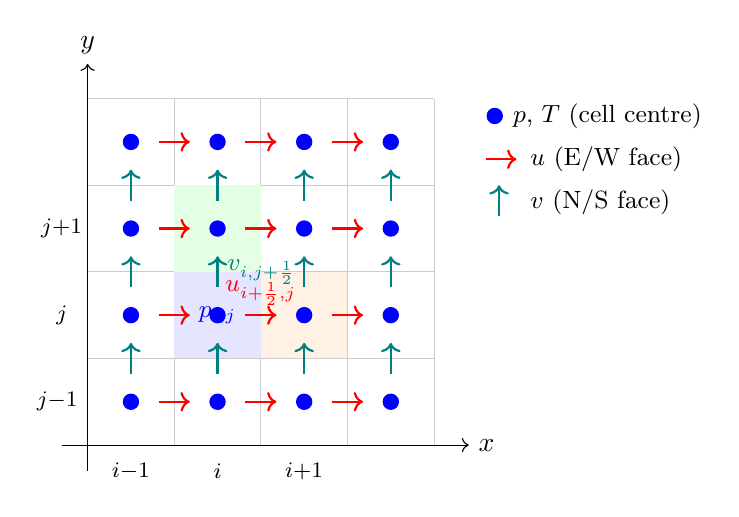
\begin{tikzpicture}[scale=1.1]
    % Grid lines
    \draw[gray!40, thin] (0,0) grid (4,4);

    % Highlight one control volume for p
    \fill[blue!10] (1,1) rectangle (2,2);
    \fill[green!10] (1,2) rectangle (2,3);
    \fill[orange!10] (2,1) rectangle (3,2);

    % Cell centers (pressure / scalar)
    \foreach \i in {0.5,1.5,2.5,3.5} {
        \foreach \j in {0.5,1.5,2.5,3.5} {
            \filldraw[blue] (\i,\j) circle (2.5pt);
        }
    }
    % u-faces (east/west faces)
    \foreach \i in {1,2,3} {
        \foreach \j in {0.5,1.5,2.5,3.5} {
            \draw[red,thick,->] (\i-0.18,\j) -- (\i+0.18,\j);
        }
    }
    % v-faces (north/south faces)
    \foreach \i in {0.5,1.5,2.5,3.5} {
        \foreach \j in {1,2,3} {
            \draw[teal,thick,->] (\i,\j-0.18) -- (\i,\j+0.18);
        }
    }

    % Labels for one cell
    \node[blue, font=\small] at (1.5,1.5) {$p_{i,j}$};
    \node[red,  font=\small, above] at (2,1.5) {$u_{i+\frac{1}{2},j}$};
    \node[teal, font=\small, right] at (1.5,2) {$v_{i,j+\frac{1}{2}}$};

    % Axes
    \draw[->] (-0.3,0) -- (4.4,0) node[right]{$x$};
    \draw[->] (0,-0.3) -- (0,4.4) node[above]{$y$};

    % Index labels
    \node[font=\footnotesize] at (0.5,-0.3) {$i{-}1$};
    \node[font=\footnotesize] at (1.5,-0.3) {$i$};
    \node[font=\footnotesize] at (2.5,-0.3) {$i{+}1$};
    \node[font=\footnotesize] at (-0.35,0.5) {$j{-}1$};
    \node[font=\footnotesize] at (-0.3,1.5) {$j$};
    \node[font=\footnotesize] at (-0.3,2.5) {$j{+}1$};

    % Legend
    \filldraw[blue] (4.7,3.8) circle (2.5pt);
    \node[font=\small, right] at (4.8,3.8) {$p$, $T$ (cell centre)};
    \draw[red,thick,->] (4.6,3.3) -- (4.95,3.3);
    \node[font=\small, right] at (5.0,3.3) {$u$ (E/W face)};
    \draw[teal,thick,->] (4.75,2.65) -- (4.75,3.0);
    \node[font=\small, right] at (5.0,2.8) {$v$ (N/S face)};
\end{tikzpicture}
\caption{Staggered Cartesian grid. Scalars ($p$, $T$) sit at cell centres (blue dots); $u$ is stored on east/west faces (red arrows); $v$ on north/south faces (teal arrows).}
\label{fig:cart_grid}
\end{figure}

% ----------------------------------------------------------
\subsection{Finite Volume Discretisation --- Integration over $\Delta x\,\Delta y$}
% ----------------------------------------------------------

Each equation is integrated over the appropriate control volume (CV) of area $\Delta x\,\Delta y$.

\subsubsection{Continuity Equation}

Integrating Eq.~\eqref{eq:cart_cont} over the scalar CV centred at $(i,j)$:
\begin{equation}
    \int_{\Delta y}\!\int_{\Delta x}
    \left(\frac{\partial u}{\partial x}+\frac{\partial v}{\partial y}\right)
    dx\,dy = 0
\end{equation}

Applying the divergence theorem (face fluxes):
\begin{equation}
    \frac{u_{i+\frac{1}{2},j} - u_{i-\frac{1}{2},j}}{\Delta x}
    + \frac{v_{i,j+\frac{1}{2}} - v_{i,j-\frac{1}{2}}}{\Delta y} = 0
    \label{eq:cart_disc_cont}
\end{equation}

\subsubsection{$x$-Momentum: CV at $(i+\tfrac{1}{2},\,j)$}

Integrating Eq.~\eqref{eq:cart_momx} over $[\,x_i,\,x_{i+1}\,]\times[\,y_{j-\frac{1}{2}},\,y_{j+\frac{1}{2}}\,]$:

\textbf{Temporal term:}
\begin{equation}
    \frac{\partial u_{i+\frac{1}{2},j}}{\partial t} \approx
    \frac{u_{i+\frac{1}{2},j}^{n+1} - u_{i+\frac{1}{2},j}^{n}}{\Delta t}
\end{equation}

\textbf{Convective terms} (central differencing):
\begin{align}
    u\frac{\partial u}{\partial x}\bigg|_{i+\frac{1}{2},j}
    &\approx u_{i+\frac{1}{2},j}\,
       \frac{u_{i+\frac{3}{2},j} - u_{i-\frac{1}{2},j}}{2\,\Delta x}
    \\[4pt]
    v\frac{\partial u}{\partial y}\bigg|_{i+\frac{1}{2},j}
    &\approx \bar{v}_{i+\frac{1}{2},j}\,
       \frac{u_{i+\frac{1}{2},j+1} - u_{i+\frac{1}{2},j-1}}{2\,\Delta y}
\end{align}
where $\bar{v}_{i+\frac{1}{2},j}
= \tfrac{1}{4}\!\left(v_{i,j+\frac{1}{2}}+v_{i+1,j+\frac{1}{2}}
                     +v_{i,j-\frac{1}{2}}+v_{i+1,j-\frac{1}{2}}\right)$
is the averaged $v$ at the $u$-face.

\textbf{Pressure gradient:}
\begin{equation}
    \frac{1}{\rho}\frac{\partial p}{\partial x}\bigg|_{i+\frac{1}{2},j}
    \approx \frac{1}{\rho}\frac{p_{i+1,j} - p_{i,j}}{\Delta x}
\end{equation}

\textbf{Viscous diffusion:}
\begin{equation}
    \nu\!\left(\frac{\partial^2 u}{\partial x^2}
              +\frac{\partial^2 u}{\partial y^2}\right)_{i+\frac{1}{2},j}
    \approx \nu\!\left(
      \frac{u_{i+\frac{3}{2},j}-2u_{i+\frac{1}{2},j}+u_{i-\frac{1}{2},j}}{\Delta x^2}
      +\frac{u_{i+\frac{1}{2},j+1}-2u_{i+\frac{1}{2},j}+u_{i+\frac{1}{2},j-1}}{\Delta y^2}
    \right)
\end{equation}

\subsubsection{$y$-Momentum: CV at $(i,\,j+\tfrac{1}{2})$}

By symmetry with the $x$-momentum equation:

\textbf{Convective terms:}
\begin{align}
    u\frac{\partial v}{\partial x}\bigg|_{i,j+\frac{1}{2}}
    &\approx \bar{u}_{i,j+\frac{1}{2}}\,
       \frac{v_{i+1,j+\frac{1}{2}} - v_{i-1,j+\frac{1}{2}}}{2\,\Delta x}
    \\[4pt]
    v\frac{\partial v}{\partial y}\bigg|_{i,j+\frac{1}{2}}
    &\approx v_{i,j+\frac{1}{2}}\,
       \frac{v_{i,j+\frac{3}{2}} - v_{i,j-\frac{1}{2}}}{2\,\Delta y}
\end{align}
where $\bar{u}_{i,j+\frac{1}{2}}
= \tfrac{1}{4}\!\left(u_{i+\frac{1}{2},j}+u_{i-\frac{1}{2},j}
                     +u_{i+\frac{1}{2},j+1}+u_{i-\frac{1}{2},j+1}\right)$.

% ----------------------------------------------------------
\subsection{Projection (Pressure-Correction) Method}
% ----------------------------------------------------------

\subsubsection{Step 1 --- Predictor (intermediate velocities $u^*$, $v^*$)}

Advance the momentum equations \emph{without} the pressure gradient:

\begin{equation}
\boxed{
u^{*}_{i+\frac{1}{2},j} = u^n_{i+\frac{1}{2},j}
+ \Delta t\left[
  -u^n_{i+\frac{1}{2},j}\frac{u^n_{i+\frac{3}{2},j}-u^n_{i-\frac{1}{2},j}}{2\Delta x}
  -\bar{v}^n_{i+\frac{1}{2},j}\frac{u^n_{i+\frac{1}{2},j+1}-u^n_{i+\frac{1}{2},j-1}}{2\Delta y}
  +\nu\!\left(
    \frac{u^n_{i+\frac{3}{2},j}-2u^n_{i+\frac{1}{2},j}+u^n_{i-\frac{1}{2},j}}{\Delta x^2}
    +\frac{u^n_{i+\frac{1}{2},j+1}-2u^n_{i+\frac{1}{2},j}+u^n_{i+\frac{1}{2},j-1}}{\Delta y^2}
  \right)
\right]
}
\label{eq:cart_pred_u}
\end{equation}

\begin{equation}
\boxed{
v^{*}_{i,j+\frac{1}{2}} = v^n_{i,j+\frac{1}{2}}
+ \Delta t\left[
  -\bar{u}^n_{i,j+\frac{1}{2}}\frac{v^n_{i+1,j+\frac{1}{2}}-v^n_{i-1,j+\frac{1}{2}}}{2\Delta x}
  -v^n_{i,j+\frac{1}{2}}\frac{v^n_{i,j+\frac{3}{2}}-v^n_{i,j-\frac{1}{2}}}{2\Delta y}
  +\nu\!\left(
    \frac{v^n_{i+1,j+\frac{1}{2}}-2v^n_{i,j+\frac{1}{2}}+v^n_{i-1,j+\frac{1}{2}}}{\Delta x^2}
    +\frac{v^n_{i,j+\frac{3}{2}}-2v^n_{i,j+\frac{1}{2}}+v^n_{i,j-\frac{1}{2}}}{\Delta y^2}
  \right)
\right]
}
\label{eq:cart_pred_v}
\end{equation}

\subsubsection{Step 2 --- Poisson Equation for Pressure Correction $p'$}

Enforcing $\nabla\cdot\mathbf{u}^{n+1}=0$ after the corrector step
$\mathbf{u}^{n+1}=\mathbf{u}^*-\Delta t\,\nabla p'/\rho$
yields the Poisson equation:

\begin{equation}
    \frac{\partial^2 p'}{\partial x^2}+\frac{\partial^2 p'}{\partial y^2}
    = \frac{\rho}{\Delta t}\left(
        \frac{\partial u^*}{\partial x}+\frac{\partial v^*}{\partial y}
      \right)
    \label{eq:cart_poisson}
\end{equation}

Discretised on the scalar CV at $(i,j)$:

\begin{equation}
\boxed{
\frac{p'_{i+1,j}-2p'_{i,j}+p'_{i-1,j}}{\Delta x^2}
+\frac{p'_{i,j+1}-2p'_{i,j}+p'_{i,j-1}}{\Delta y^2}
= \frac{\rho}{\Delta t}\left(
  \frac{u^*_{i+\frac{1}{2},j}-u^*_{i-\frac{1}{2},j}}{\Delta x}
  +\frac{v^*_{i,j+\frac{1}{2}}-v^*_{i,j-\frac{1}{2}}}{\Delta y}
\right)
}
\label{eq:cart_disc_poisson}
\end{equation}

This linear system $\mathbf{A}\,\mathbf{p}'=\mathbf{b}$ is solved at every time step (see Section~\ref{sec:cart_poisson_solver}).

\subsubsection{Step 3 --- Velocity Correction}

\begin{equation}
\boxed{
    u^{n+1}_{i+\frac{1}{2},j} = u^*_{i+\frac{1}{2},j}
    - \frac{\Delta t}{\rho}\,\frac{p'_{i+1,j}-p'_{i,j}}{\Delta x}
}
\label{eq:cart_corr_u}
\end{equation}

\begin{equation}
\boxed{
    v^{n+1}_{i,j+\frac{1}{2}} = v^*_{i,j+\frac{1}{2}}
    - \frac{\Delta t}{\rho}\,\frac{p'_{i,j+1}-p'_{i,j}}{\Delta y}
}
\label{eq:cart_corr_v}
\end{equation}

\subsubsection{Step 4 --- Pressure Update}

\begin{equation}
\boxed{
    p^{n+1}_{i,j} = p^{n}_{i,j} + \zeta\,p'_{i,j}
}
\label{eq:cart_pupdate}
\end{equation}

where $\zeta \in (0,1]$ is an under-relaxation factor (commonly $\zeta = 0.5$).

% ----------------------------------------------------------
\subsection{Poisson Solver Procedure}
\label{sec:cart_poisson_solver}
% ----------------------------------------------------------

Equation~\eqref{eq:cart_disc_poisson} can be rearranged to isolate $p'_{i,j}$:

\begin{equation}
    p'_{i,j} = \frac{1}{2\!\left(\dfrac{1}{\Delta x^2}+\dfrac{1}{\Delta y^2}\right)}
    \left[
        \frac{p'_{i+1,j}+p'_{i-1,j}}{\Delta x^2}
       +\frac{p'_{i,j+1}+p'_{i,j-1}}{\Delta y^2}
       - b_{i,j}
    \right]
    \label{eq:cart_gs}
\end{equation}

where
$b_{i,j} = \dfrac{\rho}{\Delta t}
\!\left(\dfrac{u^*_{i+\frac{1}{2},j}-u^*_{i-\frac{1}{2},j}}{\Delta x}
        +\dfrac{v^*_{i,j+\frac{1}{2}}-v^*_{i,j-\frac{1}{2}}}{\Delta y}\right)$.

\textbf{Iterative procedure (Gauss--Seidel or SOR):}
\begin{enumerate}
    \item Initialise $p'_{i,j}=0$ everywhere.
    \item Apply boundary conditions for $p'$ (Neumann $\partial p'/\partial n = 0$ at walls; $p'=0$ at outflow).
    \item Sweep all interior cells using Eq.~\eqref{eq:cart_gs}: \\
          SOR version: $p'^{\,\text{new}}_{i,j} = p'^{\,\text{old}}_{i,j} + \omega\!\left(p'^{\,\text{GS}}_{i,j}-p'^{\,\text{old}}_{i,j}\right)$, with $1 < \omega < 2$.
    \item Check convergence: $\max_{i,j}|p'^{\,\text{new}}_{i,j}-p'^{\,\text{old}}_{i,j}| < \varepsilon$.
    \item Repeat from step 2 until converged.
\end{enumerate}

\textbf{Alternatively --- Direct solver (LU / sparse):}
Assemble the $(N_x N_y)\times(N_x N_y)$ sparse matrix $\mathbf{A}$ from Eq.~\eqref{eq:cart_disc_poisson} and solve $\mathbf{A}\mathbf{p}'=\mathbf{b}$ once per time step using \texttt{scipy.sparse.linalg.spsolve} (or similar).

% ----------------------------------------------------------
\subsection{Ghost Cells and Boundary Conditions}
% ----------------------------------------------------------

Ghost (halo) cells are fictitious cells added one layer outside the physical boundary.  They allow interior-stencil formulas to be applied uniformly up to the boundary without special-casing.

\begin{figure}[H]
\centering
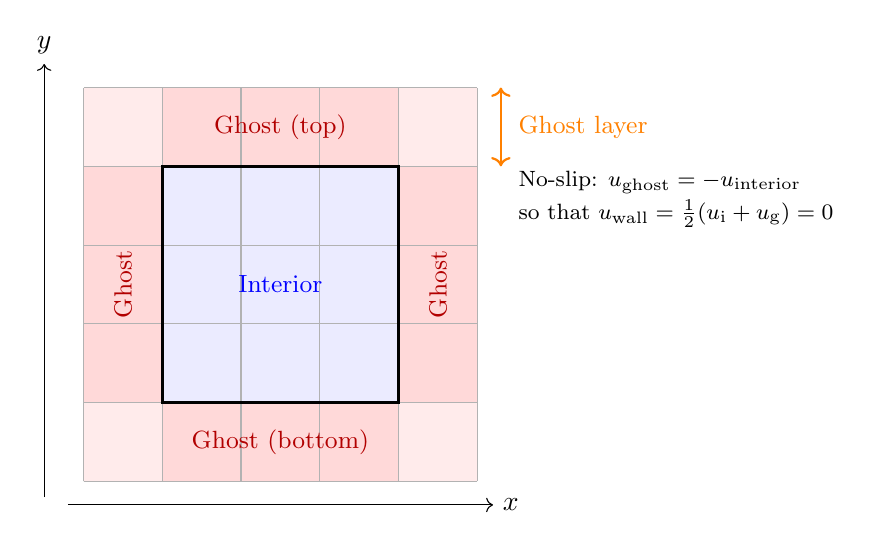
\begin{tikzpicture}[scale=1.0]
    % Physical domain (3x3 interior)
    \fill[blue!8] (1,0) rectangle (4,3);
    % Ghost cells top
    \fill[red!15] (1,3) rectangle (4,4);
    % Ghost cells bottom
    \fill[red!15] (1,-1) rectangle (4,0);
    % Ghost cells left
    \fill[red!15] (0,0) rectangle (1,3);
    % Ghost cells right
    \fill[red!15] (4,0) rectangle (5,3);
    % Ghost corners
    \fill[red!8] (0,-1) rectangle (1,0);
    \fill[red!8] (4,-1) rectangle (5,0);
    \fill[red!8] (0,3) rectangle (1,4);
    \fill[red!8] (4,3) rectangle (5,4);

    % Grid lines
    \draw[gray!60] (0,-1) grid (5,4);
    % Bold boundary
    \draw[black, very thick] (1,0) rectangle (4,3);

    % Labels
    \node[font=\small, blue] at (2.5,1.5) {Interior};
    \node[font=\small, red!70!black] at (2.5,3.5) {Ghost (top)};
    \node[font=\small, red!70!black] at (2.5,-0.5) {Ghost (bottom)};
    \node[font=\small, red!70!black, rotate=90] at (0.5,1.5) {Ghost};
    \node[font=\small, red!70!black, rotate=90] at (4.5,1.5) {Ghost};

    % BC annotation: no-slip wall at top
    \draw[<->, orange, thick] (5.3,3) -- (5.3,4);
    \node[orange, font=\small, right] at (5.4,3.5) {Ghost layer};
    \node[font=\footnotesize, right] at (5.4,2.8) {No-slip: $u_\text{ghost}=-u_\text{interior}$};
    \node[font=\footnotesize, right] at (5.4,2.4) {so that $u_\text{wall}=\tfrac{1}{2}(u_\text{i}+u_\text{g})=0$};

    % Axes
    \draw[->] (-0.2,-1.3) -- (5.2,-1.3) node[right]{$x$};
    \draw[->] (-0.5,-1.2) -- (-0.5,4.3) node[above]{$y$};
\end{tikzpicture}
\caption{Ghost cell (halo) layout for a 2D Cartesian domain. Red cells are ghost cells; blue cells are physical interior cells. The bold rectangle marks the physical boundary.}
\label{fig:cart_ghost}
\end{figure}

\textbf{How to set ghost cell values:}

\begin{center}
\begin{tabular}{llll}
\toprule
Boundary & Condition & Variable & Ghost cell value \\
\midrule
No-slip wall  & $u_w=0$, $v_w=0$  & $u$  & $u_\text{ghost} = -u_\text{interior}$ \\
              &                   & $v$  & $v_\text{ghost} = -v_\text{interior}$ \\
              & $\partial p/\partial n=0$ & $p$ & $p_\text{ghost} = p_\text{interior}$ \\
\midrule
Symmetry (e.g.\ centreline) & $\partial u/\partial y=0$ & $u$ & $u_\text{ghost} = u_\text{interior}$ \\
                             & $v=0$ & $v$ & $v_\text{ghost} = -v_\text{interior}$ \\
\midrule
Inlet & $u=U_\text{in}$, $v=0$ & $u$ & $u_\text{ghost} = 2U_\text{in}-u_\text{interior}$ \\
\midrule
Outlet (zero-gradient) & $\partial(\cdot)/\partial x=0$ & any & $\phi_\text{ghost}=\phi_\text{interior}$ \\
\bottomrule
\end{tabular}
\end{center}

The ghost cell value is computed \emph{before} each Runge--Kutta or Adams--Bashforth stage so that boundary conditions are enforced at the correct sub-step.


\newpage

% ============================================================
%  Derivation: 2D Cylindrical Coordinates (r, phi)
%  Velocities: u (radial), v (azimuthal)
%  Integration element: dr dphi   (no z-dependence)
% ============================================================

\section{2D Incompressible Flow in Cylindrical Coordinates $(r,\phi)$ --- Velocities $(u,v)$}
\label{sec:cyl_uv}

\subsection{Governing Equations (Strong Form)}

For flow in the $(r,\phi)$-plane with $\partial/\partial z = 0$ and $w = 0$:

\textbf{Continuity:}
\begin{equation}
    \frac{1}{r}\frac{\partial(ru)}{\partial r}
    +\frac{1}{r}\frac{\partial v}{\partial\phi} = 0
    \quad\Longleftrightarrow\quad
    \frac{\partial u}{\partial r}+\frac{u}{r}
    +\frac{1}{r}\frac{\partial v}{\partial\phi} = 0
    \label{eq:cyl_uv_cont}
\end{equation}

\textbf{Radial momentum ($r$-direction):}
\begin{equation}
    \frac{\partial u}{\partial t}
    + \frac{1}{r}\frac{\partial(ru^2)}{\partial r}
    + \frac{1}{r}\frac{\partial(uv)}{\partial\phi}
    - \frac{v^2}{r}
    = -\frac{1}{\rho}\frac{\partial p}{\partial r}
    + \frac{1}{\rho r}\frac{\partial(r\tau_{rr})}{\partial r}
    + \frac{1}{\rho r}\frac{\partial\tau_{r\phi}}{\partial\phi}
    - \frac{\tau_{\phi\phi}}{\rho r}
    \label{eq:cyl_uv_momr}
\end{equation}

\textbf{Azimuthal momentum ($\phi$-direction):}
\begin{equation}
    \frac{\partial v}{\partial t}
    + \frac{1}{r}\frac{\partial(ruv)}{\partial r}
    + \frac{1}{r}\frac{\partial(v^2)}{\partial\phi}
    + \frac{uv}{r}
    = -\frac{1}{\rho r}\frac{\partial p}{\partial\phi}
    + \frac{1}{\rho r}\frac{\partial(r\tau_{r\phi})}{\partial r}
    + \frac{1}{\rho r}\frac{\partial\tau_{\phi\phi}}{\partial\phi}
    \label{eq:cyl_uv_momv}
\end{equation}

where $\tau_{rr}$, $\tau_{r\phi}$, and $\tau_{\phi\phi}$ are stress tensor components. For Newtonian fluids with constant viscosity $\mu = \rho\nu$:
\begin{align}
    \tau_{rr} &= 2\mu\frac{\partial u}{\partial r}
    \\
    \tau_{r\phi} &= \mu\!\left(r\frac{\partial}{\partial r}\left(\frac{v}{r}\right)+\frac{1}{r}\frac{\partial u}{\partial\phi}\right)
    \\
    \tau_{\phi\phi} &= 2\mu\left(\frac{u}{r}+\frac{1}{r}\frac{\partial v}{\partial\phi}\right)
\end{align}

The centripetal ($-v^2/r$) and Coriolis ($+uv/r$) terms arise from the curvature of the coordinate system.

\textbf{Conservation vs.\ Convective Form:}
The equations above are in \emph{conservation form}, expressing momentum fluxes as divergences: $\frac{1}{r}\frac{\partial(ru^2)}{\partial r}$ and $\frac{1}{r}\frac{\partial(uv)}{\partial\phi}$ in the radial equation. To derive the \emph{convective form}, expand these using the product rule. For example, in the radial momentum equation:
\begin{equation}
    \frac{1}{r}\frac{\partial(ru^2)}{\partial r} + \frac{1}{r}\frac{\partial(uv)}{\partial\phi}
    = \frac{u}{r}\frac{\partial(ru)}{\partial r} + u\frac{\partial u}{\partial r} + \frac{1}{r}\frac{\partial(uv)}{\partial\phi}
    = u\left(\frac{1}{r}\frac{\partial(ru)}{\partial r} + \frac{1}{r}\frac{\partial v}{\partial\phi}\right) + u\frac{\partial u}{\partial r} + \frac{v}{r}\frac{\partial u}{\partial\phi}
\end{equation}
By continuity $\frac{1}{r}\frac{\partial(ru)}{\partial r} + \frac{1}{r}\frac{\partial v}{\partial\phi} = 0$, the grouped term vanishes:
\begin{equation}
    \frac{1}{r}\frac{\partial(ru^2)}{\partial r} + \frac{1}{r}\frac{\partial(uv)}{\partial\phi} = u\frac{\partial u}{\partial r} + \frac{v}{r}\frac{\partial u}{\partial\phi}
\end{equation}
This is the **convective form**. In cylindrical coordinates, the conservation form is essential for finite volume methods because the metric factors ($r$-weighting) appear naturally in the flux integrals. The divergence structure ensures that discrete momentum is conserved when integrated over the annular control volume with area element $r\,dr\,d\phi$.

% ----------------------------------------------------------
\subsection{Staggered Grid Layout}
% ----------------------------------------------------------

\begin{figure}[H]
\centering
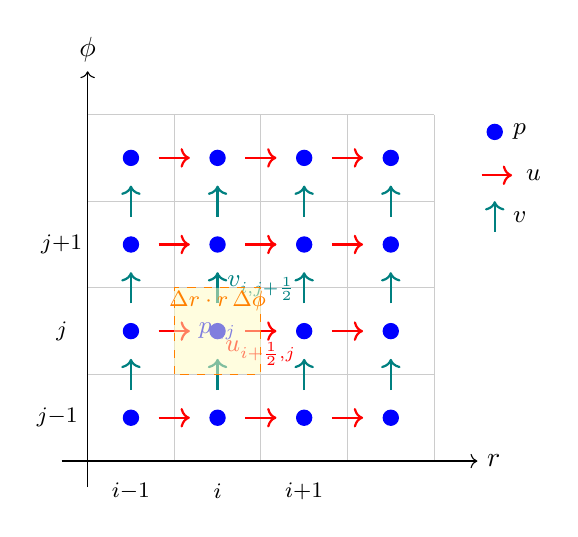
\begin{tikzpicture}[scale=1.1]
    % Grid (r horizontal, phi vertical)
    \draw[gray!40,thin] (0,0) grid (4,4);

    % Cell centres
    \foreach \i in {0.5,1.5,2.5,3.5}{
        \foreach \j in {0.5,1.5,2.5,3.5}{
            \filldraw[blue] (\i,\j) circle (2.5pt);
        }
    }
    % u-faces (radial direction, horizontal faces)
    \foreach \i in {1,2,3}{
        \foreach \j in {0.5,1.5,2.5,3.5}{
            \draw[red,thick,->] (\i-0.18,\j) -- (\i+0.18,\j);
        }
    }
    % v-faces (azimuthal direction, vertical faces)
    \foreach \i in {0.5,1.5,2.5,3.5}{
        \foreach \j in {1,2,3}{
            \draw[teal,thick,->] (\i,\j-0.18) -- (\i,\j+0.18);
        }
    }

    % Axes
    \draw[->] (-0.3,0) -- (4.5,0) node[right]{$r$};
    \draw[->] (0,-0.3) -- (0,4.5) node[above]{$\phi$};

    % Labels for one cell
    \node[blue,  font=\small] at (1.5,1.5) {$p_{i,j}$};
    \node[red,   font=\small, below] at (2,1.5) {$u_{i+\frac{1}{2},j}$};
    \node[teal,  font=\small, right] at (1.5,2) {$v_{i,j+\frac{1}{2}}$};

    % Index labels
    \node[font=\footnotesize] at (0.5,-0.35) {$i{-}1$};
    \node[font=\footnotesize] at (1.5,-0.35) {$i$};
    \node[font=\footnotesize] at (2.5,-0.35) {$i{+}1$};
    \node[font=\footnotesize] at (-0.35,0.5) {$j{-}1$};
    \node[font=\footnotesize] at (-0.3,1.5) {$j$};
    \node[font=\footnotesize] at (-0.3,2.5) {$j{+}1$};

    % Control volume sketch
    \fill[yellow!25, opacity=0.5] (1,1) rectangle (2,2);
    \draw[dashed, orange] (1,1) rectangle (2,2);
    \node[font=\footnotesize, orange] at (1.5,1.85) {$\Delta r \cdot r\,\Delta\phi$};

    % Legend
    \filldraw[blue] (4.7,3.8) circle (2.5pt); \node[font=\small,right] at (4.8,3.8) {$p$};
    \draw[red,thick,->]  (4.55,3.3) -- (4.9,3.3); \node[font=\small,right] at (4.95,3.3) {$u$};
    \draw[teal,thick,->] (4.7,2.65) -- (4.7,3.0); \node[font=\small,right] at (4.8,2.82) {$v$};
\end{tikzpicture}
\caption{Staggered grid in the $(r,\phi)$ plane. Scalars at cell centres (blue); radial velocity $u$ at $r$-faces (red); azimuthal velocity $v$ at $\phi$-faces (teal). The control volume area element is $\Delta r \cdot r\,\Delta\phi$.}
\label{fig:cyl_uv_grid}
\end{figure}

% ----------------------------------------------------------
\subsection{Finite Volume Discretisation --- Integration over $\Delta r\,(r\,\Delta\phi)$}
% ----------------------------------------------------------

The FV approach integrates the conservation laws over a discrete control volume (CV), converting PDEs into algebraic equations. The key tool is the **2D Gauss divergence theorem**:

\begin{equation}
    \iint_{\Omega} \nabla \cdot \mathbf{F} \, dA = \oint_{\partial\Omega} \mathbf{F} \cdot \mathbf{n} \, ds
\end{equation}

where $\Omega$ is the control volume, $\mathbf{F}$ is a flux vector, and $\mathbf{n}$ is the outward normal. This transforms volume integrals of divergence into surface integrals of normal fluxes, which are discretized at cell faces. This is why the **conservation form** of the equations (with divergence operators) is so natural for FV: each divergence term directly corresponds to net flux out of the cell boundaries.

\textbf{Domain:} The FV area element in the $(r,\phi)$-plane is $dA = r\,dr\,d\phi$.
Cell $(i,j)$ occupies $r\in[r_{i-\frac{1}{2}},r_{i+\frac{1}{2}}]$,
$\phi\in[\phi_{j-\frac{1}{2}},\phi_{j+\frac{1}{2}}]$.

\subsubsection{Continuity Equation}

Integrating Eq.~\eqref{eq:cyl_uv_cont} over the scalar CV:
\begin{equation}
    \int_{\phi_{j-\frac{1}{2}}}^{\phi_{j+\frac{1}{2}}}
    \int_{r_{i-\frac{1}{2}}}^{r_{i+\frac{1}{2}}}
    \left[\frac{1}{r}\frac{\partial(ru)}{\partial r}
         +\frac{1}{r}\frac{\partial v}{\partial\phi}\right]
    r\,dr\,d\phi = 0
\end{equation}

Applying the 2D divergence theorem:
\begin{equation}
\boxed{
    \frac{r_{i+\frac{1}{2}}\,u_{i+\frac{1}{2},j} - r_{i-\frac{1}{2}}\,u_{i-\frac{1}{2},j}}{r_i\,\Delta r}
    + \frac{v_{i,j+\frac{1}{2}} - v_{i,j-\frac{1}{2}}}{r_i\,\Delta\phi} = 0
}
\label{eq:cyl_uv_disc_cont}
\end{equation}

\subsubsection{Azimuthal Momentum: CV at $(i,\,j+\tfrac{1}{2})$}

Integrate Eq.~\eqref{eq:cyl_uv_momv} over $[r_{i-\frac{1}{2}},r_{i+\frac{1}{2}}]\times[\phi_j,\phi_{j+1}]$:

\textbf{Temporal term:}
\begin{equation}
    \frac{v_{i,j+\frac{1}{2}}^{n+1}-v_{i,j+\frac{1}{2}}^{n}}{\Delta t}
\end{equation}

\textbf{Convective terms:}
\begin{align}
    u\frac{\partial v}{\partial r}\bigg|_{i,j+\frac{1}{2}}
    &\approx \bar{u}_{i,j+\frac{1}{2}}\,
      \frac{v_{i+1,j+\frac{1}{2}}-v_{i-1,j+\frac{1}{2}}}{2\Delta r}
    \\[4pt]
    \frac{v}{r}\frac{\partial v}{\partial\phi}\bigg|_{i,j+\frac{1}{2}}
    &\approx \frac{v_{i,j+\frac{1}{2}}}{r_i}\,
      \frac{v_{i,j+\frac{3}{2}}-v_{i,j-\frac{1}{2}}}{2\Delta\phi}
    \\[4pt]
    \frac{uv}{r}\bigg|_{i,j+\frac{1}{2}}
    &\approx \frac{\bar{u}_{i,j+\frac{1}{2}}\,v_{i,j+\frac{1}{2}}}{r_i}
    \quad\text{(centripetal coupling term)}
\end{align}

\textbf{Pressure gradient:}
\begin{equation}
    \frac{1}{\rho r}\frac{\partial p}{\partial\phi}\bigg|_{i,j+\frac{1}{2}}
    \approx \frac{1}{\rho\,r_i}\,\frac{p_{i,j+1}-p_{i,j}}{\Delta\phi}
\end{equation}

\textbf{Viscous diffusion:}
\begin{align}
    \nu\!\left(\frac{\partial^2 v}{\partial r^2}+\frac{1}{r}\frac{\partial v}{\partial r}-\frac{v}{r^2}\right)
    &\approx \frac{\nu}{r_i\,\Delta r}\!\left(
       r_{i+\frac{1}{2}}\frac{v_{i+1,j+\frac{1}{2}}-v_{i,j+\frac{1}{2}}}{\Delta r}
      -r_{i-\frac{1}{2}}\frac{v_{i,j+\frac{1}{2}}-v_{i-1,j+\frac{1}{2}}}{\Delta r}
    \right) - \frac{\nu\,v_{i,j+\frac{1}{2}}}{r_i^2}
    \\[4pt]
    \frac{\nu}{r^2}\frac{\partial^2 v}{\partial\phi^2}
    &\approx \frac{\nu}{r_i^2}\,
      \frac{v_{i,j+\frac{3}{2}}-2v_{i,j+\frac{1}{2}}+v_{i,j-\frac{1}{2}}}{\Delta\phi^2}
    \\[4pt]
    \frac{2\nu}{r^2}\frac{\partial u}{\partial\phi}
    &\approx \frac{2\nu}{r_i^2}\,
      \frac{\bar{u}_{i,j+1}-\bar{u}_{i,j}}{\Delta\phi}
\end{align}

\subsubsection{Radial Momentum: CV at $(i+\tfrac{1}{2},\,j)$}

\textbf{Convective terms:}
\begin{align}
    u\frac{\partial u}{\partial r}\bigg|_{i+\frac{1}{2},j}
    &\approx u_{i+\frac{1}{2},j}\,
      \frac{u_{i+\frac{3}{2},j}-u_{i-\frac{1}{2},j}}{2\Delta r}
    \\[4pt]
    \frac{v}{r}\frac{\partial u}{\partial\phi}\bigg|_{i+\frac{1}{2},j}
    &\approx \frac{\bar{v}_{i+\frac{1}{2},j}}{r_{i+\frac{1}{2}}}\,
      \frac{u_{i+\frac{1}{2},j+1}-u_{i+\frac{1}{2},j-1}}{2\Delta\phi}
    \\[4pt]
    \frac{v^2}{r}\bigg|_{i+\frac{1}{2},j}
    &\approx \frac{\bar{v}_{i+\frac{1}{2},j}^2}{r_{i+\frac{1}{2}}}
    \quad\text{(centrifugal term)}
\end{align}

\textbf{Pressure gradient:}
\begin{equation}
    \frac{1}{\rho}\frac{\partial p}{\partial r}\bigg|_{i+\frac{1}{2},j}
    \approx \frac{1}{\rho}\,\frac{p_{i+1,j}-p_{i,j}}{\Delta r}
\end{equation}

% ----------------------------------------------------------
\subsection{Projection Method}
% ----------------------------------------------------------

\subsubsection{Step 1 --- Predictor (without pressure)}

\begin{equation}
\boxed{
v^{*}_{i,j+\frac{1}{2}} = v^n_{i,j+\frac{1}{2}}
+\Delta t\left[
  -\bar{u}^n\frac{v^n_{i+1,j+\frac{1}{2}}-v^n_{i-1,j+\frac{1}{2}}}{2\Delta r}
  -\frac{v^n_{i,j+\frac{1}{2}}}{r_i}\frac{v^n_{i,j+\frac{3}{2}}-v^n_{i,j-\frac{1}{2}}}{2\Delta\phi}
  -\frac{\bar{u}^n v^n_{i,j+\frac{1}{2}}}{r_i}
  +\nu D_r^v + \nu D_\phi^v
\right]
}
\label{eq:cyl_uv_pred_v}
\end{equation}

\begin{equation}
\boxed{
u^{*}_{i+\frac{1}{2},j} = u^n_{i+\frac{1}{2},j}
+\Delta t\left[
  -u^n_{i+\frac{1}{2},j}\frac{u^n_{i+\frac{3}{2},j}-u^n_{i-\frac{1}{2},j}}{2\Delta r}
  -\frac{\bar{v}^n}{r_{i+\frac{1}{2}}}\frac{u^n_{i+\frac{1}{2},j+1}-u^n_{i+\frac{1}{2},j-1}}{2\Delta\phi}
  +\frac{(\bar{v}^n)^2}{r_{i+\frac{1}{2}}}
  +\nu D_r^u + \nu D_\phi^u
\right]
}
\label{eq:cyl_uv_pred_u}
\end{equation}

with diffusion operators:
\begin{align}
    D_r^v &= \frac{r_{i+\frac{1}{2}}(v^n_{i+1,j+\frac{1}{2}}-v^n_{i,j+\frac{1}{2}})-r_{i-\frac{1}{2}}(v^n_{i,j+\frac{1}{2}}-v^n_{i-1,j+\frac{1}{2}})}{r_i\,\Delta r^2}
            -\frac{v^n_{i,j+\frac{1}{2}}}{r_i^2}
    \\[4pt]
    D_\phi^v &= \frac{v^n_{i,j+\frac{3}{2}}-2v^n_{i,j+\frac{1}{2}}+v^n_{i,j-\frac{1}{2}}}{r_i^2\,\Delta\phi^2}
               +\frac{2}{r_i^2}\frac{\bar{u}^n_{i,j+1}-\bar{u}^n_{i,j}}{\Delta\phi}
\end{align}

\subsubsection{Step 2 --- Poisson Equation for Pressure Correction $p'$}

From $\nabla\cdot\mathbf{u}^{n+1}=0$ with $\mathbf{u}^{n+1}=\mathbf{u}^*-(\Delta t/\rho)\nabla p'$:
\begin{equation}
    \frac{1}{r}\frac{\partial}{\partial r}\!\left(r\frac{\partial p'}{\partial r}\right)
    +\frac{1}{r^2}\frac{\partial^2 p'}{\partial\phi^2}
    = \frac{\rho}{\Delta t}\left(
       \frac{1}{r}\frac{\partial(ru^*)}{\partial r}
      +\frac{1}{r}\frac{\partial v^*}{\partial\phi}
      \right)
\end{equation}

Discretised at cell $(i,j)$:
\begin{equation}
\boxed{
\frac{r_{i+\frac{1}{2}}(p'_{i+1,j}-p'_{i,j})-r_{i-\frac{1}{2}}(p'_{i,j}-p'_{i-1,j})}{r_i\,\Delta r^2}
+\frac{p'_{i,j+1}-2p'_{i,j}+p'_{i,j-1}}{r_i^2\,\Delta\phi^2}
= \frac{\rho}{\Delta t}\left(
  \frac{r_{i+\frac{1}{2}}\,u^*_{i+\frac{1}{2},j}-r_{i-\frac{1}{2}}\,u^*_{i-\frac{1}{2},j}}{r_i\,\Delta r}
  +\frac{v^*_{i,j+\frac{1}{2}}-v^*_{i,j-\frac{1}{2}}}{r_i\,\Delta\phi}
\right)
}
\label{eq:cyl_uv_disc_poisson}
\end{equation}

\subsubsection{Step 3 --- Velocity Correction}

The corrected velocities enforce discrete continuity:

\begin{equation}
\boxed{
    u^{n+1}_{i+\frac{1}{2},j} = u^*_{i+\frac{1}{2},j}
    - \frac{\Delta t}{\rho}\,\frac{p'_{i+1,j}-p'_{i,j}}{\Delta r}
}
\label{eq:cyl_uv_corr_u}
\end{equation}

\begin{equation}
\boxed{
    v^{n+1}_{i,j+\frac{1}{2}} = v^*_{i,j+\frac{1}{2}}
    - \frac{\Delta t}{\rho}\,\frac{1}{r_i}\,\frac{p'_{i,j+1}-p'_{i,j}}{\Delta\phi}
    = v^*_{i,j+\frac{1}{2}}
    - \frac{\Delta t}{\rho}\,\frac{2}{r_i}\,
      \frac{p'_{i,j+1}-p'_{i,j}}{\phi_{j+1}-\phi_{j-1}}
}
\label{eq:cyl_uv_corr_v}
\end{equation}

Note: $\phi_{j+1}-\phi_{j-1} = 2\Delta\phi$, confirming both forms are equivalent.

\subsubsection{Step 4 --- Pressure Update}

\begin{equation}
\boxed{
    p^{n+1}_{i,j} = p^{n}_{i,j} + \zeta\,p'_{i,j}, \qquad \zeta \approx 0.5
}
\label{eq:cyl_uv_pupdate}
\end{equation}

% ----------------------------------------------------------
\subsection{Poisson Solver Procedure}
% ----------------------------------------------------------

Rearranging Eq.~\eqref{eq:cyl_uv_disc_poisson}:
\begin{equation}
    p'_{i,j} = \frac{b_{i,j}
      - \dfrac{r_{i+\frac{1}{2}}\,p'_{i+1,j}+r_{i-\frac{1}{2}}\,p'_{i-1,j}}{r_i\,\Delta r^2}
      - \dfrac{p'_{i,j+1}+p'_{i,j-1}}{r_i^2\,\Delta\phi^2}
    }
    {-\dfrac{r_{i+\frac{1}{2}}+r_{i-\frac{1}{2}}}{r_i\,\Delta r^2}
     -\dfrac{2}{r_i^2\,\Delta\phi^2}}
    \label{eq:cyl_uv_gs}
\end{equation}

\textbf{Iterative procedure:}
\begin{enumerate}
    \item Initialise $p'=0$.
    \item Enforce BCs: $\partial p'/\partial r=0$ at $r=r_\text{min}$ and $r=r_\text{max}$;
          periodic in $\phi$ (or $p'=0$ at one reference point to fix the null space).
    \item Sweep interior with Eq.~\eqref{eq:cyl_uv_gs}; apply SOR with $\omega \approx 1.5$.
    \item Repeat until $\max|p'^{\text{new}}-p'^{\text{old}}|<\varepsilon$.
\end{enumerate}

\textbf{Note on periodicity:} For a full annulus ($\phi\in[0,2\pi]$) the domain is periodic in $\phi$, so no ghost cells are needed in the $\phi$-direction; instead, the first and last $\phi$-slices are identified.

% ----------------------------------------------------------
\subsection{Ghost Cells and Boundary Conditions}
% ----------------------------------------------------------

\begin{figure}[H]
\centering
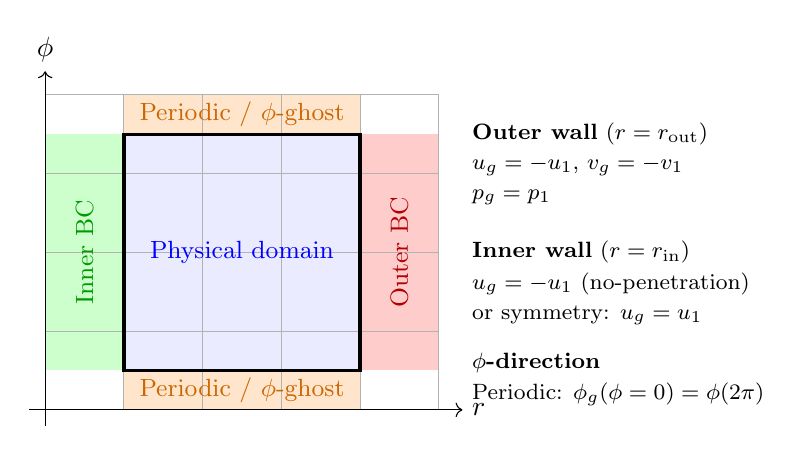
\begin{tikzpicture}[scale=1.0]
    % Physical: annular sector (displayed as rectangle r-phi)
    \fill[blue!8]  (1,0.5) rectangle (4,3.5);
    % Ghost: inner radius
    \fill[green!20] (0,0.5) rectangle (1,3.5);
    % Ghost: outer radius
    \fill[red!20]  (4,0.5) rectangle (5,3.5);
    % Ghost/periodic: phi min
    \fill[orange!20] (1,0) rectangle (4,0.5);
    % Ghost/periodic: phi max
    \fill[orange!20] (1,3.5) rectangle (4,4);

    % Grid
    \draw[gray!60,thin] (0,0) grid (5,4);
    \draw[black,very thick] (1,0.5) rectangle (4,3.5);

    % Axes
    \draw[->] (-0.2,0) -- (5.3,0) node[right]{$r$};
    \draw[->] (0,-0.2) -- (0,4.3) node[above]{$\phi$};

    % Labels
    \node[blue, font=\small] at (2.5,2)   {Physical domain};
    \node[green!60!black, font=\small, rotate=90] at (0.5,2) {Inner BC};
    \node[red!70!black, font=\small, rotate=90]   at (4.5,2) {Outer BC};
    \node[orange!80!black, font=\small] at (2.5,0.25) {Periodic / $\phi$-ghost};
    \node[orange!80!black, font=\small] at (2.5,3.75) {Periodic / $\phi$-ghost};

    % Annotations
    \node[font=\footnotesize, right] at (5.3,3.5) {\textbf{Outer wall} ($r=r_\text{out}$)};
    \node[font=\footnotesize, right] at (5.3,3.1) {$u_g=-u_1$, $v_g=-v_1$};
    \node[font=\footnotesize, right] at (5.3,2.7) {$p_g=p_1$};

    \node[font=\footnotesize, right] at (5.3,2.0) {\textbf{Inner wall} ($r=r_\text{in}$)};
    \node[font=\footnotesize, right] at (5.3,1.6) {$u_g=-u_1$ (no-penetration)};
    \node[font=\footnotesize, right] at (5.3,1.2) {or symmetry: $u_g=u_1$};

    \node[font=\footnotesize, right] at (5.3,0.6) {\textbf{$\phi$-direction}};
    \node[font=\footnotesize, right] at (5.3,0.2) {Periodic: $\phi_g(\phi=0)=\phi(2\pi)$};
\end{tikzpicture}
\caption{Ghost cell layout for the $(r,\phi)$ domain shown as a flattened rectangle. Green: inner radial BC; red: outer radial BC; orange: azimuthal boundary (periodic for a full annulus).}
\label{fig:cyl_uv_ghost}
\end{figure}

\begin{center}
\begin{tabular}{llll}
\toprule
Boundary & Condition & Variable & Ghost value \\
\midrule
Inner wall ($r=r_\text{in}$)  & No-slip: $u=0$, $v=0$  & $u$ & $u_g = -u_1$ \\
                               &                        & $v$ & $v_g = -v_1$ \\
                               & $\partial p/\partial r=0$ & $p$ & $p_g = p_1$ \\
\midrule
Outer wall ($r=r_\text{out}$) & No-slip: $u=0$, $v=0$  & $u$ & $u_g = -u_1$ \\
                               &                        & $v$ & $v_g = -v_1$ \\
                               & $\partial p/\partial r=0$ & $p$ & $p_g = p_1$ \\
\midrule
Azimuthal ($\phi$, full annulus) & Periodic & any $\phi_f$ & $\phi_g(\phi=0) = \phi_f(\phi=2\pi)$ \\
\midrule
Symmetry axis ($r=0$, if present) & $u=0$, $\partial v/\partial r=0$ & $u$ & $u_g=-u_1$ \\
                                   &                                   & $v$ & $v_g = v_1$ \\
\bottomrule
\end{tabular}
\end{center}

\subsubsection{Summary of Correction Equations (all three cases)}

For quick reference, the velocity correction equations for all three coordinate systems are:

\begin{center}
\renewcommand{\arraystretch}{2.0}
\begin{tabular}{lll}
\toprule
System & $u$-correction & $v$ (or $w$)-correction \\
\midrule
Cartesian $(x,y)$
  & $u^{n+1}_{i+\frac{1}{2},j} = u^*_{i+\frac{1}{2},j} - \dfrac{\Delta t}{\rho}\dfrac{p'_{i+1,j}-p'_{i,j}}{\Delta x}$
  & $v^{n+1}_{i,j+\frac{1}{2}} = v^*_{i,j+\frac{1}{2}} - \dfrac{\Delta t}{\rho}\dfrac{p'_{i,j+1}-p'_{i,j}}{\Delta y}$ \\[6pt]
Cylindrical $(r,z)$
  & $u^{n+1}_{i+\frac{1}{2},j} = u^*_{i+\frac{1}{2},j} - \dfrac{\Delta t}{\rho}\dfrac{p'_{i+1,j}-p'_{i,j}}{\Delta r}$
  & $w^{n+1}_{i,j+\frac{1}{2}} = w^*_{i,j+\frac{1}{2}} - \dfrac{\Delta t}{\rho}\dfrac{p'_{i,j+1}-p'_{i,j}}{\Delta z}$ \\[6pt]
Cylindrical $(r,\phi)$
  & $u^{n+1}_{i+\frac{1}{2},j} = u^*_{i+\frac{1}{2},j} - \dfrac{\Delta t}{\rho}\dfrac{p'_{i+1,j}-p'_{i,j}}{\Delta r}$
  & $v^{n+1}_{i,j+\frac{1}{2}} = v^*_{i,j+\frac{1}{2}} - \dfrac{\Delta t}{\rho}\dfrac{2}{r_i}\dfrac{p'_{i,j+1}-p'_{i,j}}{\phi_{j+1}-\phi_{j-1}}$ \\
\bottomrule
\end{tabular}
\end{center}

The extra $1/r_i$ factor in the $(r,\phi)$ case reflects the metric coefficient of the azimuthal gradient.


\end{document}
